\documentclass[11pt]{article}

% Change "review" to "final" to generate the final (sometimes called camera-ready) version.
% Change to "preprint" to generate a non-anonymous version with page numbers.

% IMPORTANT: Removed [review] so authors become visible
\usepackage{acl}

\usepackage{times}
\usepackage{latexsym}
\usepackage[T1]{fontenc}
\usepackage[utf8]{inputenc}
\usepackage{microtype}
\usepackage{inconsolata}
\usepackage{graphicx}
\usepackage{amsmath}
\usepackage{graphicx}

\title{Mapping Urban Change in Nuremberg with Machine Learning}

\setlength\titlebox{5cm}

\setlength\titlebox{5cm}

% \author{
% \textbf{Joswin Dsouza$^{*}$ \hspace{0.3cm} Macallyster Edmondson$^{*}$ \hspace{0.3cm} Praveen Narayan Hegde$^{*}$}\\ 
% \textbf{Vaibhav Prajapati$^{}$ \thanks{Authors listed in alphabetical order}}\\
% {Technische Universität Nürnberg (UTN), Germany }
% }

\author{
  Joswin Dsouza\thanks{Authors listed in alphabetical order} \quad
  Macallyster Edmondson\footnotemark[1] \quad
  Praveen Narayan Hegde\footnotemark[1] \quad
  Vaibhav Prajapati\footnotemark[1] \\
  Technische Universität Nürnberg, Germany \\
  \texttt{\{joswin.dsouza, macallyster.edmondson, praveen.narayan.hegde, vaibhav.prajapati\}@utn.de}
}

%\author{
%  \textbf{First Author\textsuperscript{1}},
%  \textbf{Second Author\textsuperscript{1,2}},
%  \textbf{Third T. Author\textsuperscript{1}},
%  \textbf{Fourth Author\textsuperscript{1}},
%\\
%  \textbf{Fifth Author\textsuperscript{1,2}},
%  \textbf{Sixth Author\textsuperscript{1}},
%  \textbf{Seventh Author\textsuperscript{1}},
%  \textbf{Eighth Author \textsuperscript{1,2,3,4}},
%\\
%  \textbf{Ninth Author\textsuperscript{1}},
%  \textbf{Tenth Author\textsuperscript{1}},
%  \textbf{Eleventh E. Author\textsuperscript{1,2,3,4,5}},
%  \textbf{Twelfth Author\textsuperscript{1}},
%\\
%  \textbf{Thirteenth Author\textsuperscript{3}},
%  \textbf{Fourteenth F. Author\textsuperscript{2,4}},
%  \textbf{Fifteenth Author\textsuperscript{1}},
%  \textbf{Sixteenth Author\textsuperscript{1}},
%\\
%  \textbf{Seventeenth S. Author\textsuperscript{4,5}},
%  \textbf{Eighteenth Author\textsuperscript{3,4}},
%  \textbf{Nineteenth N. Author\textsuperscript{2,5}},
%  \textbf{Twentieth Author\textsuperscript{1}}
%\\
%\\
%  \textsuperscript{1}Affiliation 1,
%  \textsuperscript{2}Affiliation 2,
%  \textsuperscript{3}Affiliation 3,
%  \textsuperscript{4}Affiliation 4,
%  \textsuperscript{5}Affiliation 5
%\\
%  \small{
%    \textbf{Correspondence:} \href{mailto:email@domain}{email@domain}
%  }
%}

\begin{document}
\maketitle
\begin{abstract}
Urban land-cover change, driven by built-up expansion, vegetation dynamics, and water variability, presents significant challenges for reliable modeling from satellite imagery. In this work, we propose a tabular machine learning framework for predicting land-cover composition and temporal change in Nuremberg using multi-temporal Sentinel-2 imagery and ESA WorldCover labels. We construct spatially aligned grid-based representations and design domain-informed features, including spectral indices, temporal differences, and neighborhood-based context. We evaluate both interpretable linear models and nonlinear approaches such as Random Forest, XGBoost, KNN, and a stacking ensemble. Experimental results show that ensemble-based methods outperform linear baselines, with the stacking regressor achieving the best performance (Test $R^2$ = 0.888, RMSE = 0.118) and strong classification consistency (F1 = 0.932). These results demonstrate that feature-engineered tabular models can effectively capture urban and vegetation dynamics while remaining computationally efficient and interpretable. Finally, we present an interactive dashboard that enables intuitive visualization of predicted land-cover composition, change patterns, and model confidence for non-expert users.
\end{abstract}

\section{Introduction}

Understanding urban land-cover dynamics is critical for urban planning, environmental monitoring, and policy-making \citep{seto2011global, angel2011making}. Processes such as urban expansion, vegetation loss, and infrastructure development directly impact sustainability and climate resilience. Satellite imagery provides scalable and consistent means of observing these changes \citep{wulder2018landsat, drusch2012sentinel2}, but transforming raw geospatial data into reliable and interpretable insights remains a challenging machine learning problem. Recent advances in machine learning have significantly improved remote sensing analysis \citep{li2021remote}.
In particular, convolutional neural networks (CNNs) have achieved strong performance by leveraging spatial structure in imagery \citep{zhu2017deeplearning}. However, these models often require substantial computational resources and lack interpretability, limiting their applicability in real-world decision-making scenarios \citep{samek2017explainable}. In contrast, tabular machine learning models offer a more efficient and interpretable alternative, especially when combined with engineered features \citep{grinsztajn2022tree, shwartz2022tabular}.
In this work, we investigate whether tabular models can effectively predict land-cover composition and change using multi-temporal Sentinel-2 imagery \citep{Sentinel2} and ESA WorldCover labels \citep{ESA_WorldCover}. A key challenge lies in bridging the gap between raw satellite imagery and fixed-length feature representations required by tabular models. This is further complicated by inconsistencies in spatial resolution across spectral bands \citep{roy2014landsat}, which require careful alignment and aggregation.
Our contributions to address these issues are as follows:
\begin{itemize}
    \item We propose a tabular machine learning framework for modeling urban land-cover composition and change.
    \item We incorporated domain-informed features capturing spectral, temporal, and spatial patterns.
    \item We performed comprehensive evaluation using regression, classification, and change-specific metrics.
    \item We conducted post hoc analysis of model and feature interpretability using SHAP.
    \item We developed an interactive dashboard for visualizing predictions, uncertainty, and spatial patterns.
\end{itemize}

\paragraph{Intended Users} The proposed system is designed to support non-expert stakeholders such as urban planners, sustainability analysts, and policy-makers by providing interpretable insights into land-cover dynamics. Rather than focusing on pixel-level precision, the approach emphasizes capturing broad spatial and temporal trends, enabling intuitive understanding of urban expansion, vegetation change, and water dynamics. This makes the system suitable for decision support and exploratory analysis, while acknowledging that it is not intended to replace high-resolution surveys or official land-use assessments.

\begin{figure}[h]
    \centering
    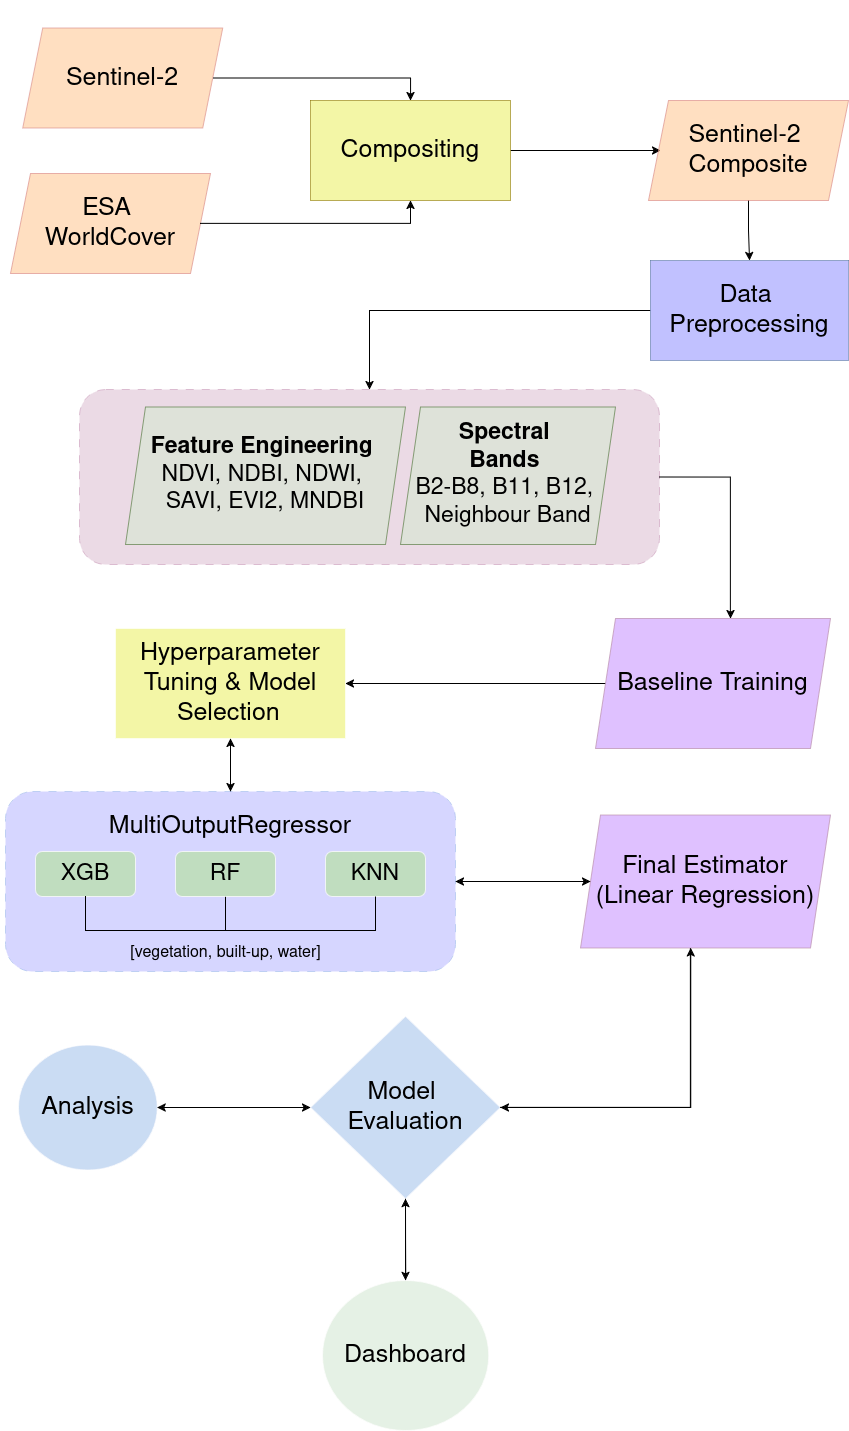
\includegraphics[width=1.0\columnwidth]{Images/ML_project.drawio.png}
    \caption{Architecture of the stacked multi-output regression model used in the final system. XGBoost, Random Forest, and KNN act as base learners, while Linear Regression serves as the final estimator within a MultiOutputRegressor framework.}
    \label{fig:architecture}
\end{figure}

\section{Method}

Urban land-cover modeling can be formulated as a structured prediction problem over spatial grid cells, where the objective is to estimate land-cover composition and its temporal evolution. Figure~\ref{fig:architecture} illustrates the overall pipeline of our approach, including data preprocessing, feature engineering, model training, and evaluation.

\subsection{Problem Framing \& Scope}

We formulate urban land-cover analysis as a supervised multi-output regression problem over spatial grid cells. Each grid cell represents a fixed spatial unit for which the model predicts the proportional composition of land-cover classes (built-up, vegetation, and water), as well as their temporal change between consecutive years.

To construct a consistent representation, the study area is discretized into regular grid cells of size $20 \times 20$ meters. This resolution is chosen as a trade-off between spatial detail and computational efficiency: it is sufficiently fine-grained to capture local urban structures while enabling aggregation of multi-spectral bands with differing resolutions (10m and 20m) into a unified representation. This design also aligns with the native resolution of key Sentinel-2 bands, minimizing information loss during resampling.

The temporal setup leverages multi-year Sentinel-2 imagery (2016–2021) for feature generation, while land-cover labels from 2020 and 2021 are used to define prediction targets. The primary task is to estimate land-cover composition at a target time step and derive land-cover change as the difference in class proportions across time.

This formulation enables the model to capture both spatial patterns and temporal dynamics of urban environments, while remaining compatible with tabular machine learning methods.

\subsection{Dataset Curation \& Preprocessing}
\paragraph{Multi-Spectral Data Integration}
We utilize multi-spectral Sentinel-2 imagery \citep{Sentinel2} (bands B1–B12) as the primary input data source \citep{drusch2012sentinel}.Ground truth labels are obtained from the ESA WorldCover dataset, which offers globally consistent land-cover maps at high spatial resolution \citep{zanaga2021worldcover}. 
 The data is accessed and processed through the Google Earth Engine \citep{GEE} platform, which provides scalable and efficient retrieval of satellite imagery. 

\subsection*{Non-trivial data issues}
\paragraph{Cloud Cover and missing data} Addressed by using images througout the year which had no greater than 20\% cloud coverage, as determined by ESA Image metadata.
\paragraph{Label imbalance}For the data collected for 2020 and 2021 Land Cover of Nuremberg, majority of labels were “Built-up” and “Tree Cover”. As we’re only training on data for the Nuremberg Metropolitan area, we chose to group some of the labels under “Vegetation”, this included “Tree Cover”, “Grassland”, and “Cropland”.This provided better performance on multi-regression accuracy.
\paragraph{Label noise in land-cover maps (We chose not to address this issue.)} The accuracy of land-cover data from ESA World Cover for the years 2020 and 2021 range from 70 -75\%. As this is the primary data used for training of our model(s), this accuracy impacts our model accuracy as well. We chose not to fix this issue as the ESA World Cover labels were required to be used and fixing the inaccuracies in the given labels was not within the scope of this project.


\begin{table*}[t]
\centering
\small
\setlength{\tabcolsep}{6pt}
\renewcommand{\arraystretch}{1.15}
\begin{tabular}{ll}
\hline
\textbf{Feature} & \textbf{Description} \\
\hline

B2  & Blue (490 nm); sensitive to water and atmospheric scattering. \\
B3  & Green (560 nm); useful for vegetation and water reflectance. \\
B4  & Red (665 nm); captures chlorophyll absorption in vegetation. \\
B5  & Red-Edge 1 (705 nm); sensitive to vegetation stress. \\
B6  & Red-Edge 2 (740 nm); captures vegetation structure. \\
B7  & Red-Edge 3 (783 nm); improves vegetation monitoring. \\
B8  & NIR (842 nm); strong vegetation reflectance, biomass indicator. \\
B11 & SWIR 1 (1610 nm); sensitive to moisture and built-up areas. \\
B12 & SWIR 2 (2190 nm); useful for soil, dryness, and urban detection. \\

NDVI \citep{yangshao2016}  & Vegetation index using NIR–Red contrast; high values indicate dense vegetation. \\
NDWI \citep{mcfeeters1996ndwi}  & Water index using Green–NIR contrast; high values indicate water bodies. \\
SAVI \citep{huete1988savi}  & Soil-adjusted vegetation index reducing soil brightness effects. \\
EVI2 \citep{jiang2008evi2}  & Enhanced vegetation index reducing atmospheric and saturation effects. \\
MNDWI \citep{xu2008mndbi} & Modified water index using SWIR to suppress urban noise in water detection. \\

\hline
\end{tabular}
\caption{Sentinel-2 spectral bands and derived index features used for land-cover modeling.}
\label{tab:feature_engineering}
\end{table*}


\subsection{Feature Engineering}
Index Based Features are mathematical transformations of spectral bands designed to enhance specific land surface characteristics such as vegetation, water, and built-up areas. These indices reduce noise, normalize illumination difference, and improve seperability between land cover classes for machine learning models. 
We derived widely used spectral indices:\\
These include the Normalized Difference Vegetation Index (NDVI), Normalized Difference Water Index (NDWI), Soil Adjusted Vegetation Index (SAVI), Enhanced Vegetation Index 2 (EVI2), and Modified Normalized Difference Water Index (MNDWI). These indices are computed using combinations of Sentinel-2 spectral bands, including B2–B8 (visible and near-infrared) and B11–B12 (shortwave infrared). Each index is designed to enhance specific land-cover properties such as vegetation, built-up areas, and water bodies. Detailed descriptions and interpretations of these features are summarized in Table~\ref{tab:feature_engineering}.

\paragraph{Neighborhood Band Features.}
To incorporate local spatial context, we augment each grid cell with spectral values from its neighboring cells. Let $B_k(x,y)$ denote the value of spectral band $k$ at spatial location $(x,y)$. For a relative offset $(\Delta x, \Delta y)$, we define a neighborhood feature as
\[
\phi_{k,\Delta x,\Delta y}(x,y) = B_k(x+\Delta x,\; y+\Delta y),
\]
where $k$ indexes the spectral band, and $\Delta x, \Delta y \in \mathbb{Z}$ represent horizontal and vertical displacements, respectively.

We adopt a consistent naming convention of the form \texttt{B\{k\}\_\{s\_x a\}\_\{s\_y b\}}, where $s_x, s_y \in \{p,m\}$ indicate positive or negative offsets and $a, b \geq 0$ denote their magnitudes. For example, \texttt{B4\_p0\_p1} corresponds to $\phi_{4,0,+1}(x,y)$, while \texttt{B2\_m1\_p0} corresponds to $\phi_{2,-1,0}(x,y)$. In our implementation, a $3 \times 3$ spatial window is used, resulting in 8 neighboring cells per grid location ensuring consistent capture of local spatial context.

These features enable the model to capture local spatial dependencies and neighborhood structure within a tabular framework, providing an efficient alternative to convolution-based approaches.

\subsection{Model Comparison}

\noindent Table~\ref{tab:model_comparison} summarizes the performance of all evaluated models across regression and dominant-class classification metrics. The results reveal a clear progression in predictive performance as model complexity increases.

Linear models (Linear Regression and Ridge) provide consistent but limited performance, with test $R^2$ values around 0.65 and relatively higher RMSE. This indicates that purely linear relationships are insufficient to capture the complexity of land-cover dynamics. Lasso Regression further underperforms ($R^2 = 0.3640$), suggesting that strong regularization leads to underfitting and loss of important feature interactions.
Nonlinear models demonstrate substantial improvements. KNN achieves strong performance ($R^2 = 0.8617$), indicating that local feature similarity is informative for land-cover prediction, although its sensitivity to noise and high-dimensional features limits robustness. Random Forest provides stable and consistent performance ($R^2 = 0.8416$), effectively capturing nonlinear interactions while maintaining generalization.
XGBoost emerges as the strongest individual model, achieving the highest test $R^2$ of 0.8759 and lowest RMSE of 0.1250. Its gradient boosting framework enables it to model complex feature interactions and subtle variations in land-cover patterns \citep{chen2016xgboost, grinsztajn2022tree}. These results suggest that different models capture complementary aspects of the data: local structure (KNN), ensemble averaging (Random Forest), and boosted optimization (XGBoost).
Motivated by this observation, we construct a stacking regressor to combine the strengths of multiple base learners. Specifically, XGBoost, Random Forest, and KNN are used as base models, while a linear regressor serves as the final estimator. This design allows the model to integrate diverse predictive signals while maintaining interpretability at the meta-learning level.
The stacking model achieves the best overall performance, with a test $R^2$ of 0.8882 and RMSE of 0.1184, along with the highest classification metrics (Accuracy = 0.9320, F1 = 0.9318). The improvement over individual models indicates that combining complementary learners enhances generalization and robustness.
Overall, these results demonstrate that while individual nonlinear models are strong predictors, their combination through stacking provides a more comprehensive representation of urban land-cover dynamics. 

\subsection{Hyperparameter Optimization}

Hyperparameter optimization was performed using Optuna, a Bayesian optimization framework that efficiently explores the search space to identify high-performing configurations \citep{akiba2019optunanextgenerationhyperparameteroptimization}. Different models were assigned model-specific search spaces and trial budgets to account for differences in training cost and complexity.
The final model configurations were selected based on validation performance, balancing predictive accuracy and computational efficiency. Table~\ref{tab:hyperparameters} summarizes the optimized hyperparameters used in the final evaluation. These tuned configurations ensure that each model operates under near-optimal conditions, enabling a fair and robust comparison.

\begin{table*}[t]
\centering
\small
\setlength{\tabcolsep}{5pt}
\renewcommand{\arraystretch}{1.1}
\begin{tabular}{ll}
\hline
\textbf{Model} & \textbf{Optimized Hyperparameters} \\
\hline

KNN & $k=28$, weights=uniform, metric=Minkowski ($p=2$), leaf\_size=24 \\

Random Forest & n\_estimators=390, max\_depth=9, min\_samples\_split=14, min\_samples\_leaf=8, max\_features=0.61 \\

XGBoost & n\_estimators=600, learning\_rate=0.0448, max\_depth=10, gamma=1.01, min\_child\_weight=11, \\
         & reg\_alpha=6.71, reg\_lambda=0.70, colsample\_bytree=0.70, subsample=0.69 \\

\hline
\end{tabular}
\caption{Optimized hyperparameters obtained using Optuna for key nonlinear models.}
\label{tab:hyperparameters}
\end{table*}

\section{Evaluation Beyond Accuracy}
\subsection{Hold-out Strategy} We used a temporal hold-out strategy in which models were trained using earlier-year information and evaluated on later-year labels. This design is more realistic than random mixing of observations because it better reflects the intended use case of predicting future land-cover composition and change. Where relevant, we also considered spatial separation effects, since neighboring grid cells are highly correlated and can otherwise inflate apparent performance.

\begin{figure}[t]
    \centering
    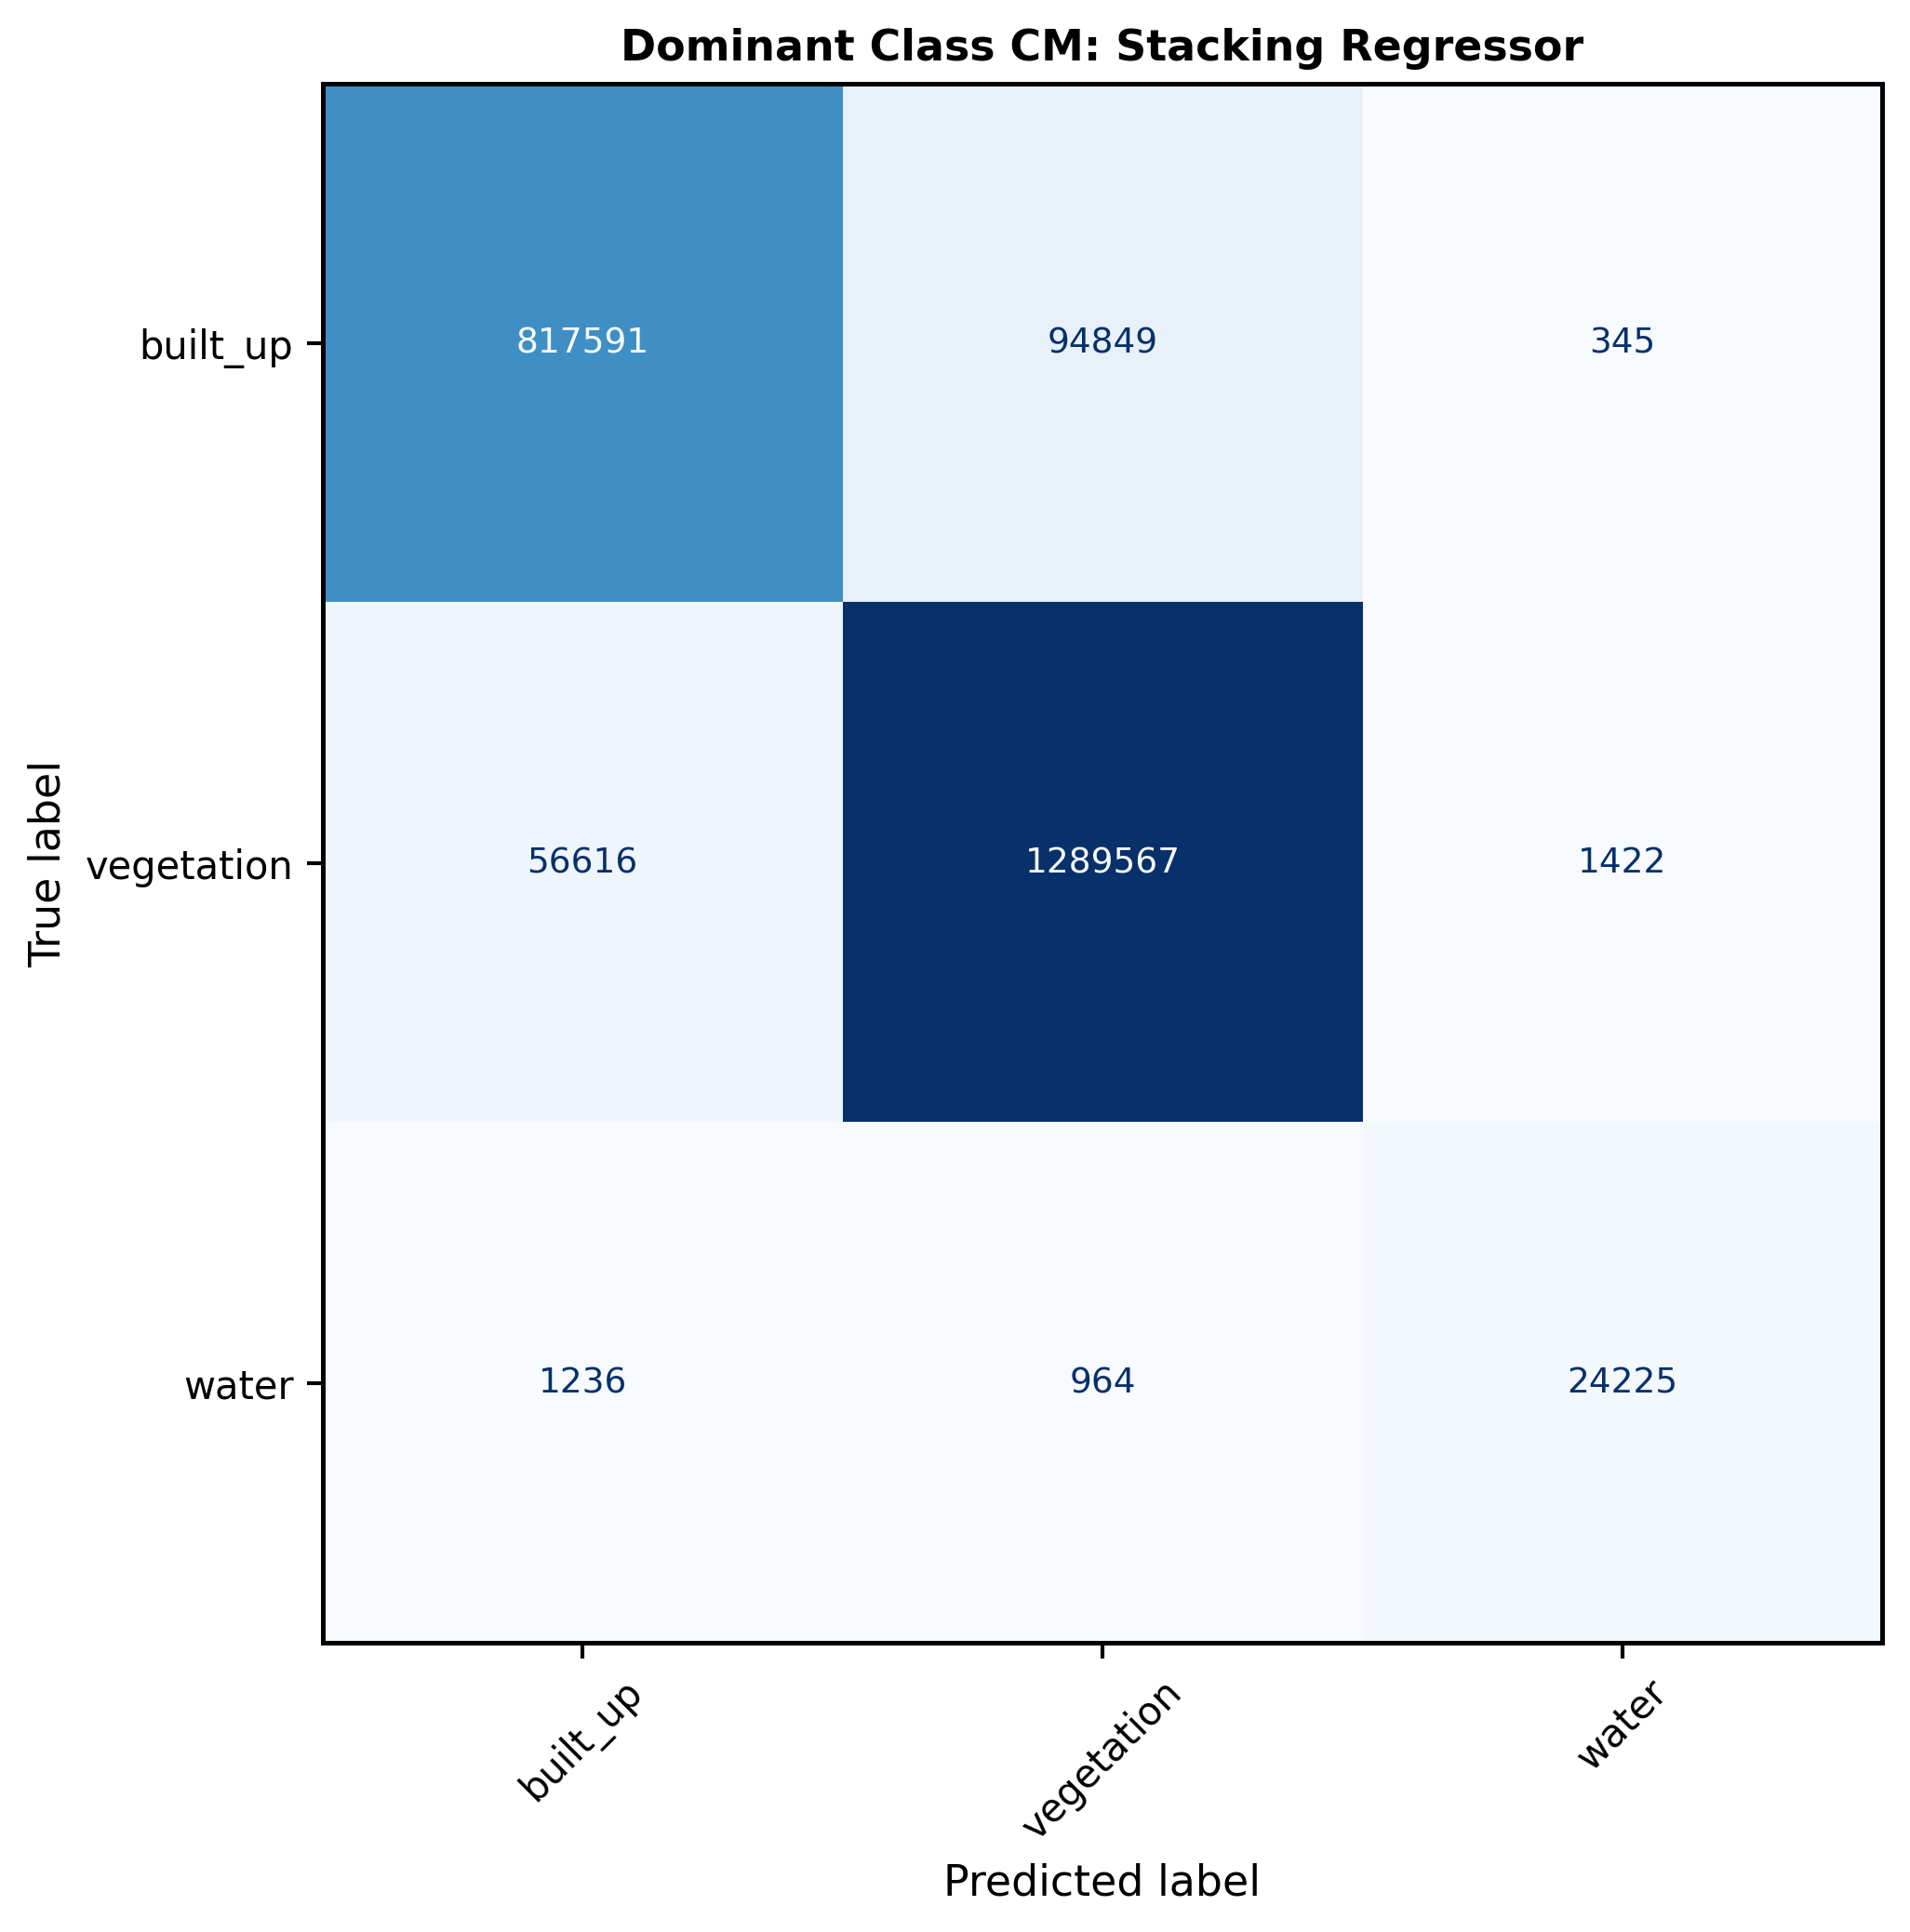
\includegraphics[width=1.0\columnwidth]{Images/cm_stacking_regressor.png}
    \caption{Confusion matrix of dominant land-cover class predictions produced by the Stacking Regressor model.}
    \label{fig:confusion_matrix}
\end{figure}

\begin{table*}[t]
\centering
\small
\setlength{\tabcolsep}{6pt}
\renewcommand{\arraystretch}{1.2}
\begin{tabular}{lcccccc}
\hline
 & \multicolumn{4}{c}{\textbf{Regression Metrics}} & \multicolumn{2}{c}{\textbf{Dominant-Class Metrics}} \\
\cline{2-5} \cline{6-7}
\textbf{Model} & Train $R^2$ & Test $R^2$ & Train RMSE & Test RMSE & Accuracy & F1-score \\
\hline
Linear Regression & 0.6599 & 0.6566 & 0.1799 & 0.1866 & 0.8935 & 0.8917 \\
Ridge Regression  & 0.6586 & 0.6557 & 0.1803 & 0.1868 & 0.8949 & 0.8932 \\
Lasso Regression  & 0.3754 & 0.3640 & 0.2262 & 0.2356 & 0.8386 & 0.8308 \\
KNN               & 0.8849 & 0.8617 & 0.1202 & 0.1334 & 0.9146 & 0.9136 \\
Random Forest     & 0.8560 & 0.8416 & 0.1331 & 0.1428 & 0.9116 & 0.9113 \\
XGBoost           & \textbf{0.8981} & \textbf{0.8759} & \textbf{0.1106} & \textbf{0.1250} & \textbf{0.9264} & \textbf{0.9262} \\
Stacking Regressor & \textbf{0.9151} & \textbf{0.8882} & \textbf{0.1016} & \textbf{0.1184} & \textbf{0.9320} & \textbf{0.9318} \\
\hline
\end{tabular}
\caption{Comparison of model performance across regression and classification metrics. 
The Stacking Regressor achieves the best overall performance.}
\label{tab:model_comparison}
\end{table*}




% -----------------------------------------------------------Single column table start--------------------------------------------------------------------------
% \begin{table}[t]
% \centering
% \small
% \setlength{\tabcolsep}{3pt}
% \begin{tabular}{lcccccc}
% \hline
%  & \multicolumn{4}{c}{\textbf{Regression}} & \multicolumn{2}{c}{\textbf{Classification}} \\
% \cline{2-5} \cline{6-7}
% \textbf{Model} & Tr $R^2$ & Te $R^2$ & Tr RMSE & Te RMSE & Acc & F1 \\
% \hline
% Linear & 0.6599 & 0.6566 & 0.1799 & 0.1866 & 0.8935 & 0.8917 \\
% Ridge  & 0.6586 & 0.6557 & 0.1803 & 0.1868 & 0.8949 & 0.8932 \\
% Lasso  & 0.3754 & 0.3640 & 0.2262 & 0.2356 & 0.8386 & 0.8308 \\
% KNN    & 0.8849 & 0.8617 & 0.1202 & 0.1334 & 0.9146 & 0.9136 \\
% RF     & 0.8560 & 0.8416 & 0.1331 & 0.1428 & 0.9116 & 0.9113 \\
% Stack  & {0.9151} & {0.8882} & {0.1016} & {0.1184} & {0.9320} & {0.9318} \\
% XGB    & \textbf{0.8981} & \textbf{0.8759} & \textbf{0.1106} & \textbf{0.1250} & \textbf{0.9264} & \textbf{0.9262} \\
% \hline
% \end{tabular}
% \caption{Comparison of model performance across regression and classification metrics. \\
% Tr = Train, Te = Test, Acc = Accuracy, F1 = F1-score.}
% \label{tab:model_comparison}
% \end{table}

% -----------------------------------------------------------Single column table end--------------------------------------------------------------------------





\subsection{Stress Testing and Robustness Analysis}

To evaluate the robustness of the proposed system, we conducted stress tests by introducing controlled perturbations to the input features. Adding noise to inputs is a well-established approach for assessing model robustness and has been shown to act as a form of regularization in machine learning models \citep{bishop1995training}.This analysis focuses on the Stack Regressor model, which demonstrated strong performance in previous evaluations.



\paragraph{Gaussian Noise Injection}
To evaluate robustness under realistic perturbations, we inject Gaussian noise into the input features at levels of 5\%, 10\%, and 25\%, simulating sensor noise and environmental variability commonly present in satellite imagery \citep{zhu2017deep}.

Table~\ref{tab:noise_results} shows that model performance degrades progressively with increasing noise. At low noise levels (5\%), the model maintains strong predictive accuracy with only minor reductions in $R^2$ and slight increases in RMSE, indicating robustness to small perturbations. At moderate noise (10\%), performance declines more noticeably but remains stable, suggesting that the learned feature representations capture resilient patterns.

\begin{table}[h] \centering \resizebox{\columnwidth}{!}{ \begin{tabular}{lcccc} \hline \textbf{Noise Level} & \textbf{Train $R^2$} & \textbf{Test $R^2$} & \textbf{Train RMSE} & \textbf{Test RMSE} \\ \hline 5\% & 0.8926 & 0.8719 & 0.1136 & 0.1273 \\ 10\% & 0.8830 & 0.8629 & 0.1189 & 0.1320 \\ 25\% & 0.8237 & 0.8070 & 0.1467 & 0.1575 \\ \hline \end{tabular} } \caption{Model performance under increasing levels of Gaussian noise with XGBoost.} \label{tab:noise_results} \end{table}

Under high noise (25\%), a larger drop in performance is observed ($R^2 = 0.8070$), reflecting increased sensitivity to severe perturbations. However, the degradation remains gradual, and the model retains reasonable predictive capability. The consistent gap between training and test performance across all noise levels indicates stable generalization.
Overall, these results demonstrate that the proposed feature-engineered framework captures robust relationships and maintains reliability under noisy input conditions, which is critical for real-world remote sensing applications \citep{hendrycks2019benchmarking}.

% \subsection{Error Analysis}
% Error analysis revealed that the most difficult cells were located in mixed-use transition regions, especially along boundaries between built-up and vegetation-dominated areas. These regions often contain heterogeneous land cover within a single grid cell, making both labels and predictions less reliable. Seasonal effects also introduced ambiguity: temporary vegetation changes could resemble genuine land-cover conversion, and this sometimes led the model to overestimate vegetation loss or urban expansion. Water detection was generally more robust, likely because NDWI provides a clearer spectral signal than the separation between sparse vegetation and built-up surfaces.

\subsection{Analysis and Interpretability}
To better understand the behavior of our models, we analyze performance across temporal horizons and investigate feature importance using SHAP values \citep{lundberg2017unified}. The following analysis focuses on the Stack Regressor model, which demonstrated strong predictive performance among the evaluated methods.

\paragraph{Performance Across Temporal Horizons}
We evaluate model performance across different temporal prediction horizons, defined by the time gap $\Delta$ (in years) between input features and target labels. Figures~\ref{fig:RMSE} and~\ref{fig:r2} present RMSE and $R^2$ scores for both training and test sets.

\begin{figure}[h] \centering 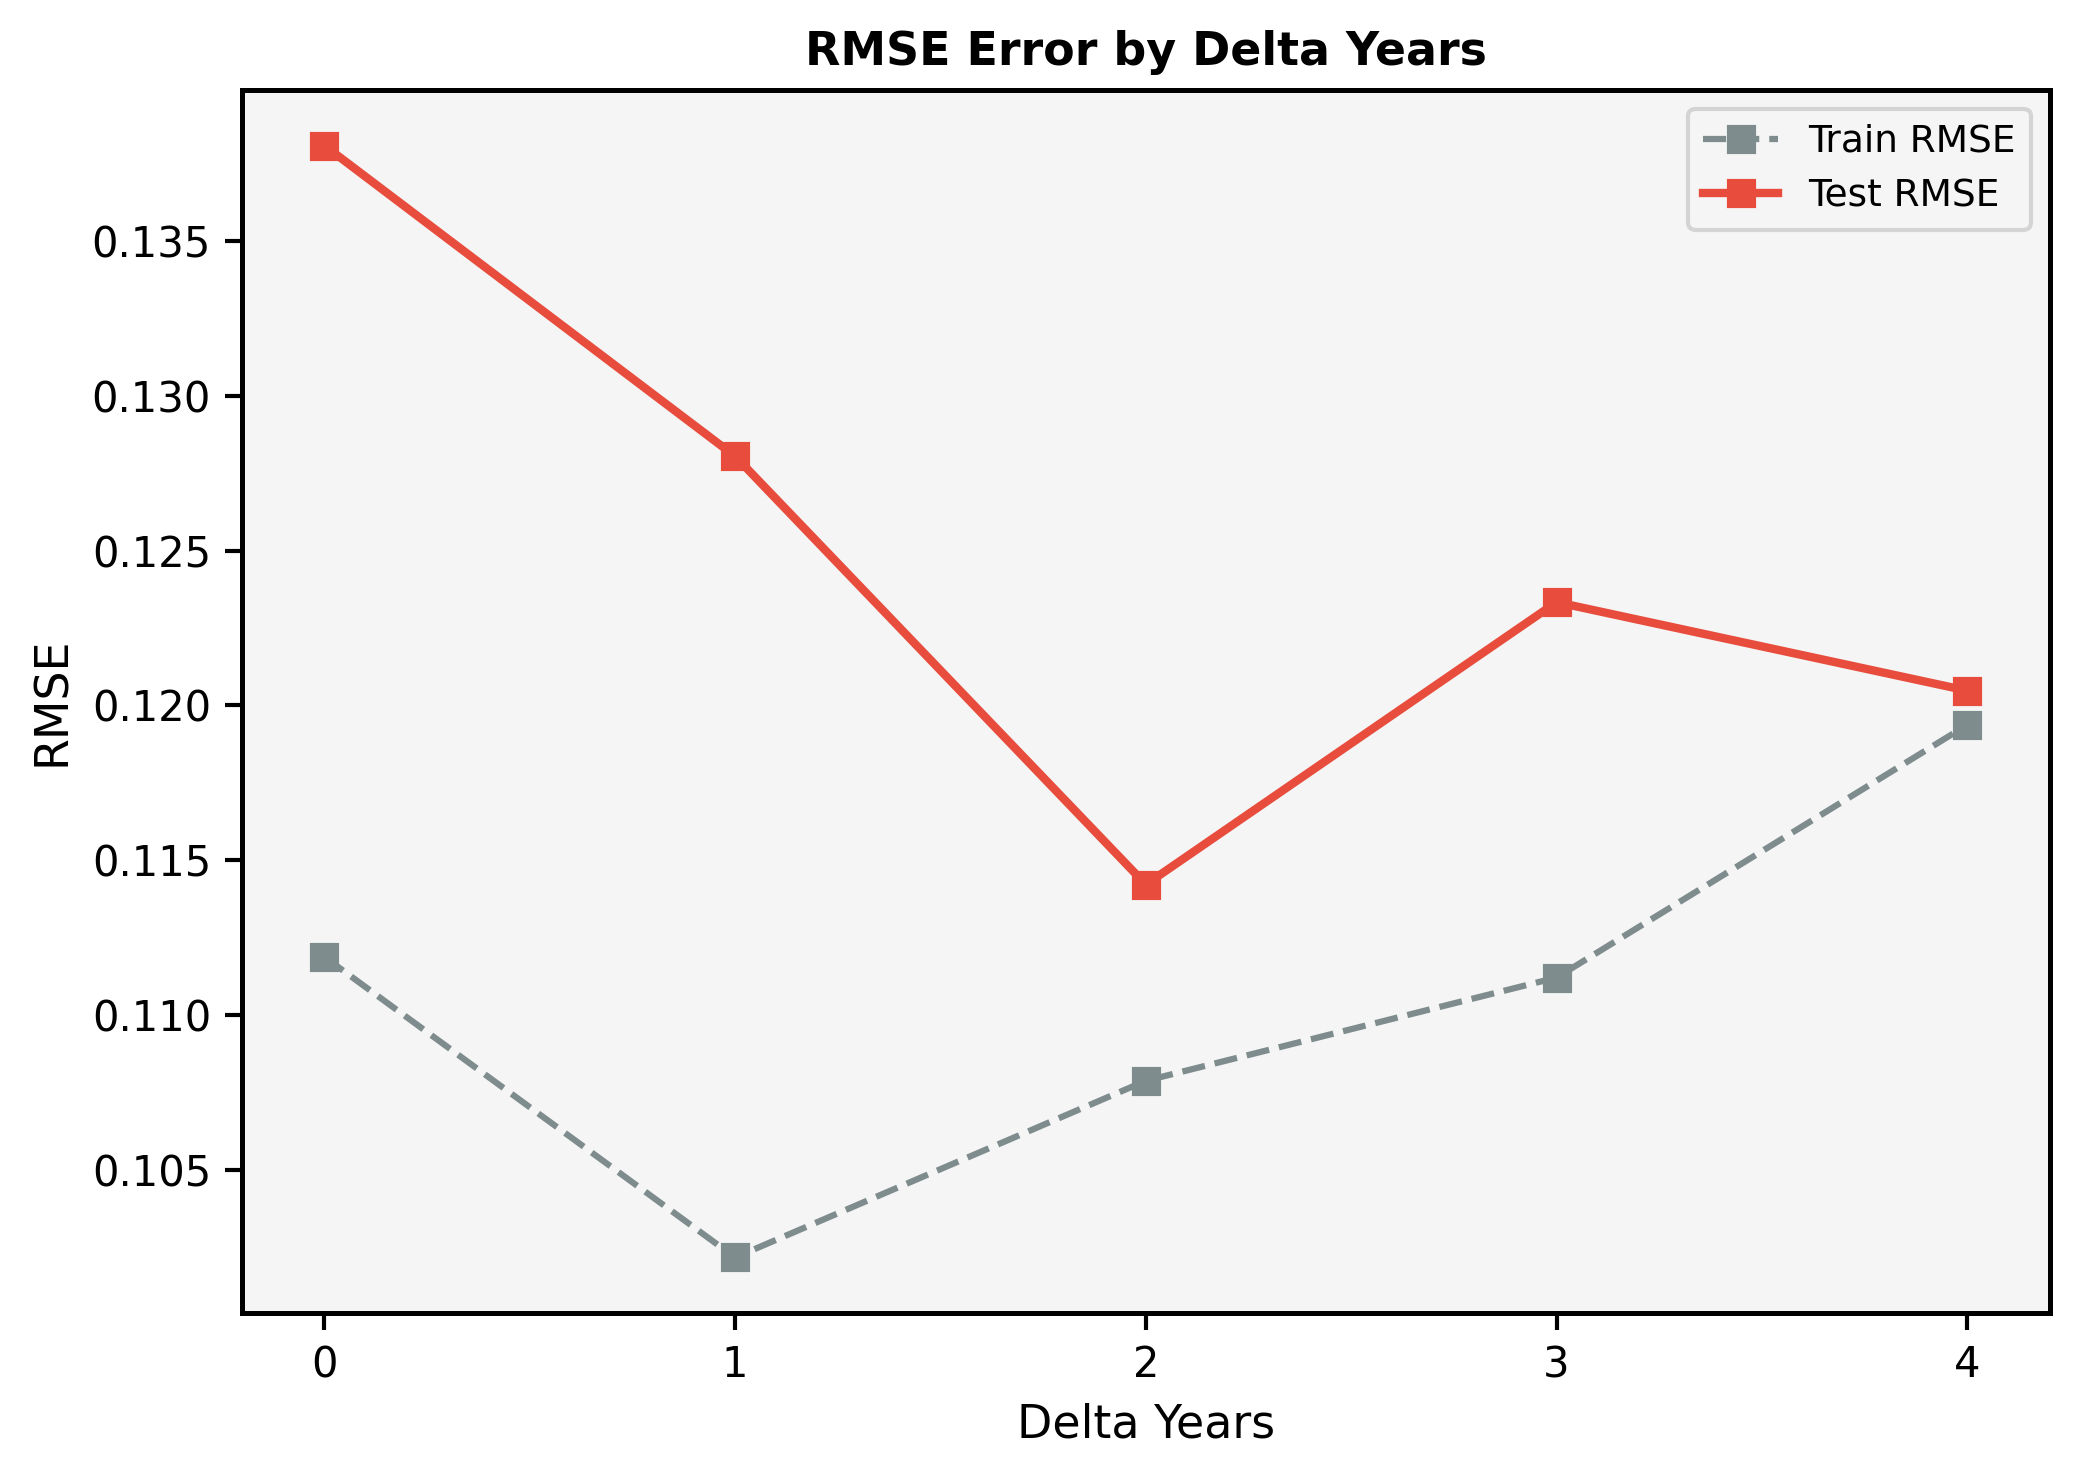
\includegraphics[width=1.0\columnwidth]{Images/rmse_error_per_delta.png} \caption{RMSE across different temporal horizons ($\Delta$ years) with XGBoost.} \label{fig:RMSE} \end{figure}
\begin{figure}[h] \centering 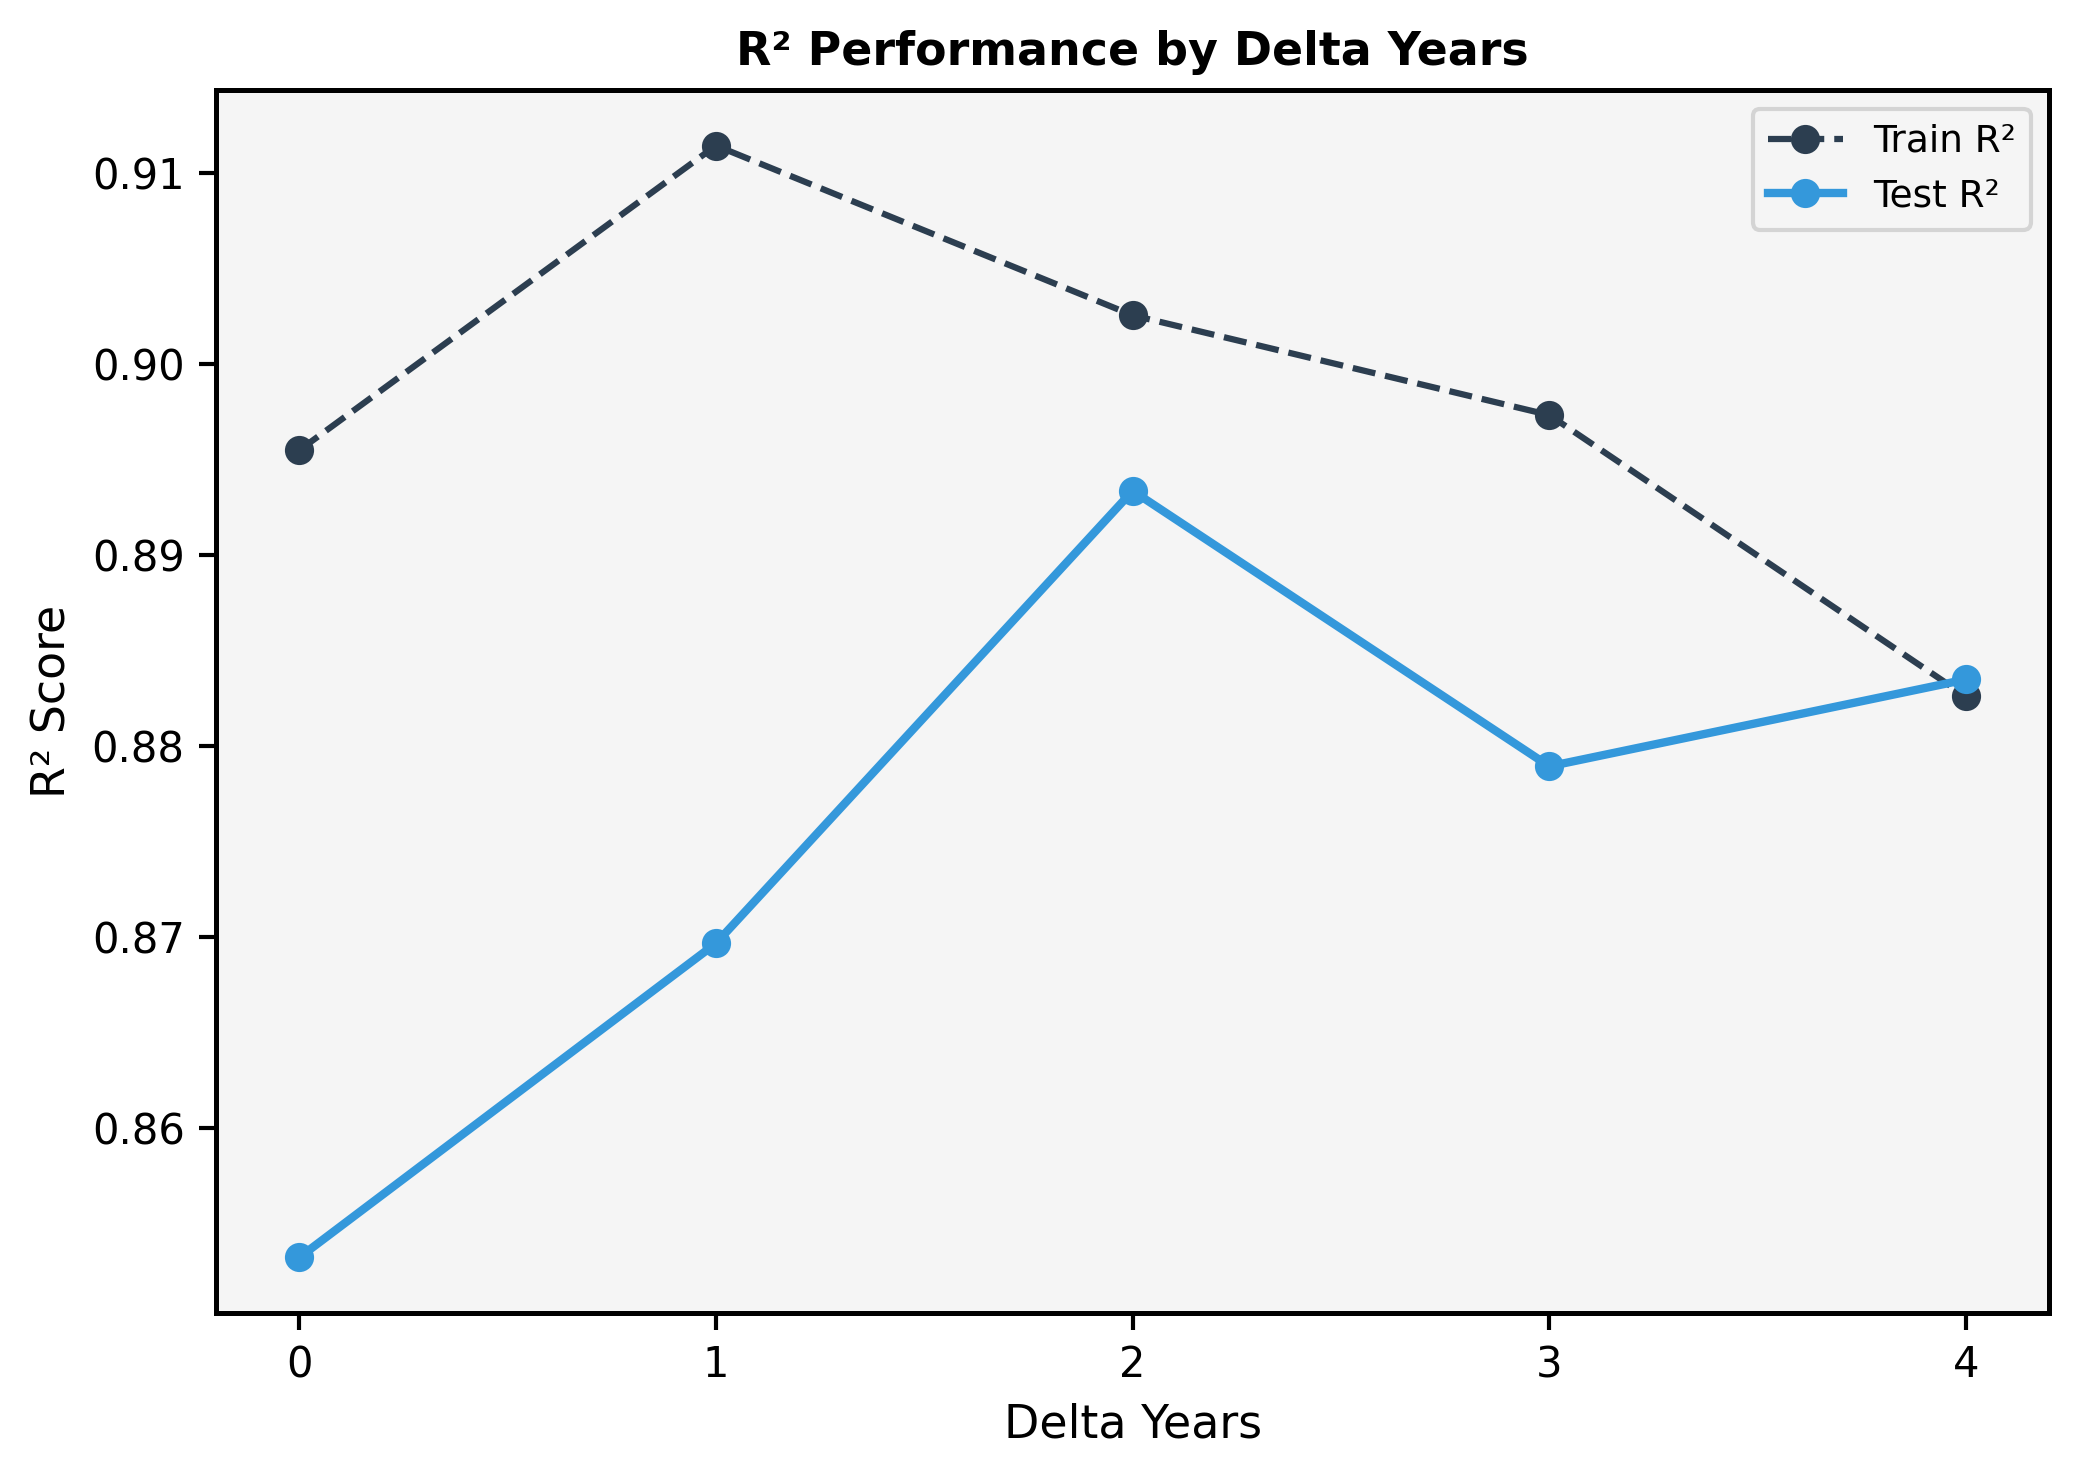
\includegraphics[width=1.0\columnwidth]{Images/r2_performance_per_delta.png} \caption{$R^2$ performance across different temporal horizons ($\Delta$ years) with XGBoost.} \label{fig:r2} \end{figure}


The results show that predictive performance is optimal at $\Delta = 2$, where the model achieves the lowest RMSE and highest $R^2$. This indicates that short-to-mid-term temporal dependencies are effectively captured by the feature set. 

At $\Delta = 0$, performance is comparatively weaker, with higher RMSE and lower $R^2$. This can be attributed to short-term variability in satellite observations, including noise, seasonal fluctuations, and inconsistencies in label generation, which reduce predictability at immediate time scales.

For larger temporal gaps ($\Delta \geq 3$), performance gradually degrades, reflected by increasing RMSE and declining $R^2$. This suggests that long-term land-cover dynamics are influenced by additional factors not captured by the current feature representation, leading to increased uncertainty.

Overall, these results indicate that the model is most reliable for moderate temporal horizons, while both short-term noise and long-term uncertainty limit predictive performance.

\paragraph{Feature Importance Analysis}

To interpret the contribution of different features, we use SHAP (SHapley Additive exPlanations) values computed for the Stacking Regressor model using Permutation Explainer. Figure~\ref{fig:feature} shows the top 12 most influential features based on mean absolute SHAP values.

\begin{figure}[h]
    \centering
    
\includegraphics[width=1.0\columnwidth]{Images/global_feature_importance.png}
    \caption{Top 12 features influencing model predictions based on SHAP values with Stacking Regressor.}
    \label{fig:feature}
\end{figure}

The results indicate that vegetation-related indices, particularly EVI2 and SAVI, are the most influential features. This highlights the importance of vegetation dynamics in modeling land-cover composition and change in urban environments. Traditional indices such as NDVI also contribute significantly, confirming their relevance in distinguishing vegetation from built-up areas.
In addition to spectral indices, raw neighbor spectral bands (e.g., B4\_p0\_p1, B8\_p0\_p1, etc.) and temporal features such as $\Delta$ years also play an important role. The presence of $\Delta$ years among the top features suggests that the temporal gap itself influences prediction difficulty and model behavior.
Water-related indices such as NDWI and MNDWI contribute less compared to vegetation indices, which is consistent with the relatively smaller proportion and variability of water bodies in the study area.
Overall, the feature importance analysis confirms that the model relies on physically meaningful and interpretable features, reinforcing the validity of the feature engineering design.

\paragraph{SHAP-Based Feature Interpretation}

To interpret model behavior, we analyze SHAP summary plots for individual land-cover classes. SHAP values quantify feature contributions to model predictions, where positive values increase the predicted output and negative values decrease it, with color indicating feature magnitude.

\begin{figure}[t]
\centering

\includegraphics[width=1.0\columnwidth]{Images/shap_summary_vegetation.png}
\caption{SHAP summary plot for the vegetation class with Stacking Regressor.}
\label{fig:SHAPVegetation}
\end{figure}

\begin{figure}[h]
\centering

\includegraphics[width=1.0\columnwidth]{Images/shap_summary_built_up.png}
\caption{SHAP summary plot for the built-up class with Stacking Regressor.}
\label{fig:SHAPBuiltUp}
\end{figure}

Figures~\ref{fig:SHAPVegetation} and~\ref{fig:SHAPBuiltUp} reveal distinct and physically meaningful patterns across classes. For the built-up class, the temporal feature $\Delta$ years plays a significant role, with higher values contributing positively to predictions, reflecting gradual urban expansion over time. However, the spread of SHAP values indicates that temporal information alone is insufficient and must be interpreted alongside spectral features. Neighboring spectral bands, particularly B4 (red) and B8 (NIR), contribute strongly by capturing reflectance differences between urban materials and vegetation. Vegetation indices such as NDVI exhibit negative contributions, reinforcing that higher vegetation presence reduces built-up likelihood, while water-related indices (NDWI, MNDWI) show comparatively weaker influence.

For the vegetation class, spectral indices dominate model behavior. High values of EVI2 and SAVI correspond to strong positive contributions, indicating dense vegetation, while low values contribute negatively, reflecting non-vegetated regions. NDVI further supports this pattern, demonstrating consistent sensitivity to vegetation presence. Although $\Delta$ years contributes positively, its effect is less consistent compared to spectral features, suggesting that vegetation dynamics are influenced more by environmental and seasonal factors than purely temporal progression.

An interesting observation is the consistent importance of directional neighbor features (e.g., \texttt{B4\_p0\_p1}, \texttt{B8\_p0\_p1}), which capture information from specific spatial orientations. We hypothesize that this directional asymmetry may be linked to illumination and shadow effects in satellite imagery, particularly given the geographic location of Nuremberg in the Northern Hemisphere. Such patterns suggest that certain neighboring directions systematically encode shading or reflectance differences. This phenomenon is not explicitly modeled in our framework and remains an open question for future investigation.

Overall, the SHAP analysis confirms that the model leverages physically interpretable signals, with temporal features capturing gradual urban expansion and spectral indices providing robust discrimination of vegetation and land-cover composition.


\subsection{System Integration}
The trained model is integrated into an interactive dashboard for visualization and analysis. \\
Users can inspect predicted land-cover composition per grid cell
Hover-based interaction displays class percentages
The dashboard provides configurable visualization at coarser spatial resolutions (20–200, in increments of 20), relative to the model’s native 20×20 grid. This enables efficient rendering and interactive performance without significantly compromising spatial interpretability.

\section{Explainability \& Trust}

\paragraph{What the System Explains}
The proposed system provides interpretable insights into land-cover dynamics by communicating what changed, where it changed, and the associated prediction confidence. These explanations are delivered through an interactive dashboard that visualizes spatial patterns of land-cover composition and temporal change across the study region.

\paragraph{What Changed and Where}
For each grid cell, the model predicts class proportions, and changes are computed as differences across time steps. This enables identification of urban expansion, vegetation shifts, and stable regions. The spatial visualization highlights areas of significant change, allowing users to focus on regions of interest.

\paragraph{System Confidence}
To support trustworthy interpretation, the system provides confidence estimates derived from prediction consistency. These are mapped into intuitive categories: \textit{low} (50–66.6\%), \textit{medium} (66.6–83.2\%), and \textit{high} (83.2–100\%). High-confidence predictions typically correspond to regions with strong and consistent spectral signals, while lower confidence is observed in heterogeneous or mixed land-cover areas.

\paragraph{Explanation Mechanism}
The explanations are grounded in feature-level behavior. For example, increases in built-up area are typically associated with higher NDBI and lower NDVI or SAVI values, often supported by similar patterns in neighboring cells. This reflects spatial continuity and aligns with known urban expansion processes.

\paragraph{Limitations}
Despite providing intuitive explanations, the system has limitations. It relies on noisy supervision from ESA WorldCover and aggregated grid-level features, which may obscure fine-grained patterns. Additionally, confidence estimates reflect model certainty rather than ground-truth accuracy. Therefore, the system is intended for exploratory analysis and high-level decision support rather than precise or regulatory use.

\section{Final Product}

The final system is an interactive dashboard for exploring predicted land-cover composition and change across Nuremberg. It provides a map-based interface where users can inspect spatial patterns of built-up areas, vegetation, and water. Each grid cell encodes predicted class proportions, accessible through hover-based interaction, along with confidence indicators to support interpretation.

\begin{figure}[t]
    \centering
    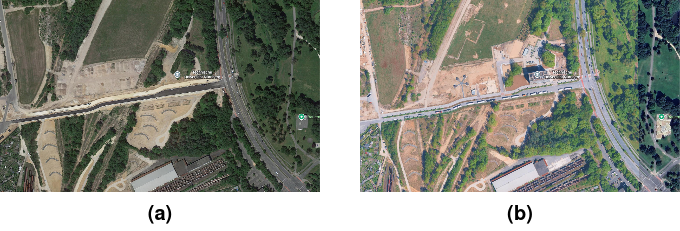
\includegraphics[width=1.0\columnwidth]{Images/UTN.drawio.png}
    \caption{Satellite imagery \citep{GoogleEarth} of the UTN campus region illustrating land-use change over time: (a) pre-development state, showing predominantly undeveloped land and sparse infrastructure; (b) post-development state, showing active construction and emerging built-up structures.}
    \label{fig:groundtruth_label}
\end{figure}

\begin{figure}[t]
    \centering
    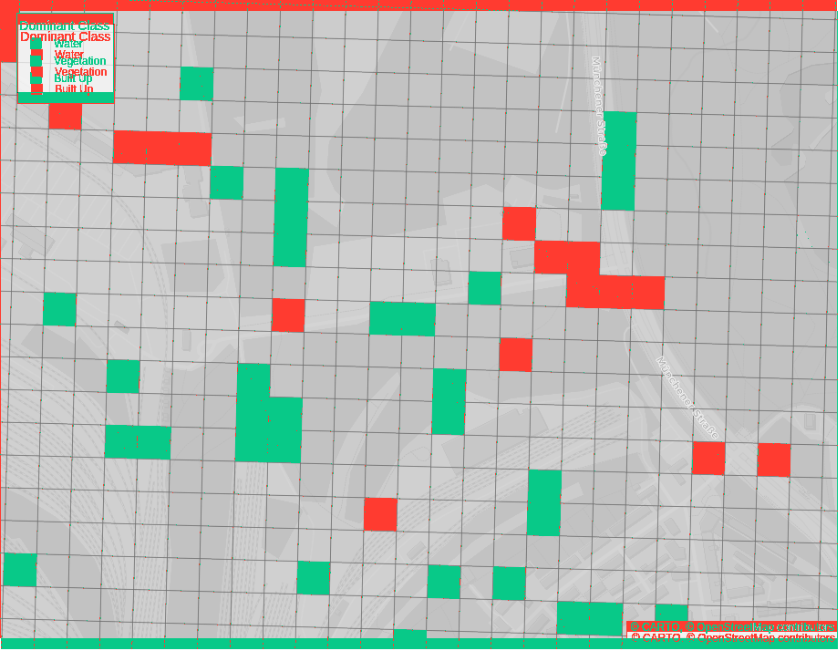
\includegraphics[width=1.0\columnwidth]{Images/UTN_Campus_diff.png}
    \caption{Model prediction for 2025 based on 2021 inputs, indicating a transition from vegetation to built-up areas in the UTN campus region.}
    \label{fig:prediction_label}
\end{figure}

\paragraph{Urban Change Detection}
Figures~\ref{fig:groundtruth_label} and~\ref{fig:prediction_label} illustrate a representative example from the UTN campus region. While the 2021 ground truth is predominantly vegetation, the model predicts a transition to built-up areas by 2025. This aligns with actual campus construction, indicating that the model captures meaningful urban expansion patterns.

\paragraph{Interpretation}
The predicted transition is supported by consistent feature patterns, including decreasing vegetation indices (NDVI, SAVI) and increasing built-up indicators, along with spatial consistency across neighboring cells. This demonstrates the model’s ability to generalize temporal dynamics without explicit future observations.

\begin{figure}[t]
    \centering
    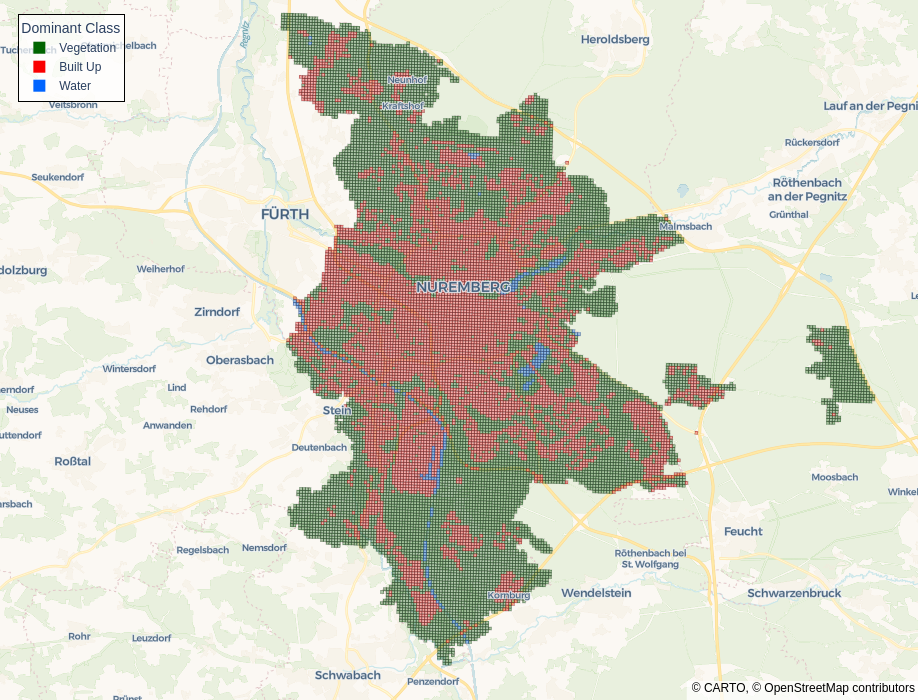
\includegraphics[width=1.0\columnwidth]{Images/2021_true_labels_100m.png}
    \caption{City-scale ground truth land-cover distribution for Nuremberg in 2021.}
    \label{fig:2021_truelabel}
\end{figure}

\begin{figure}[t]
    \centering
    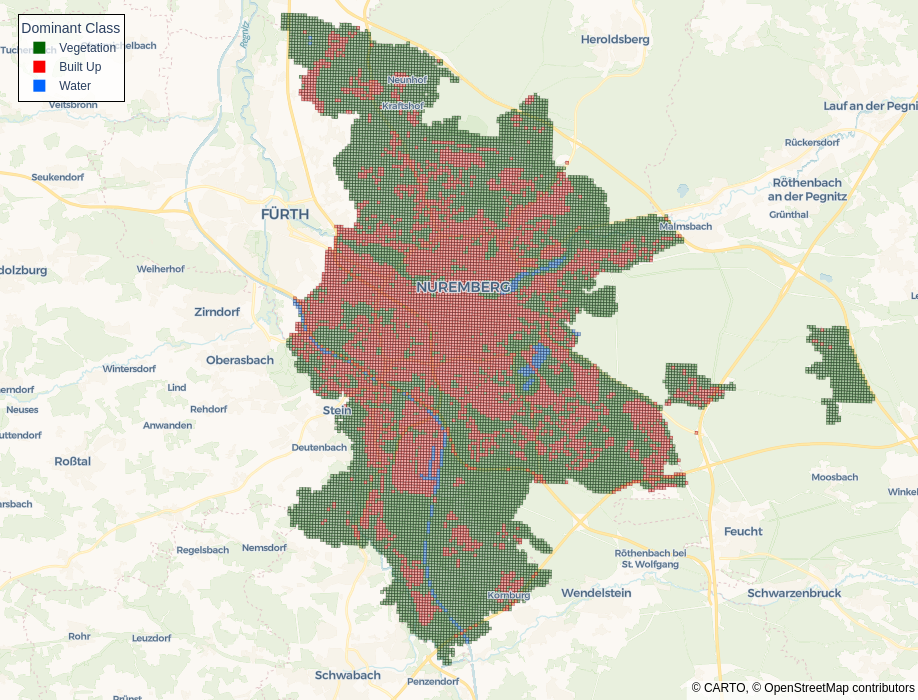
\includegraphics[width=1.0\columnwidth]{Images/2021_2019_prediction_100m.png.png}
    \caption{City-scale model predictions showing spatial distribution of dominant land-cover classes.}
    \label{fig:2019_prediction}
\end{figure}

\paragraph{City-Scale Consistency}
At the city scale (Figures~\ref{fig:2021_truelabel} and~\ref{fig:2019_prediction}), the model reproduces key spatial structures of Nuremberg. Built-up areas are concentrated in the urban core and along transport corridors, while vegetation dominates peripheral regions. The close alignment between predictions and ground truth indicates that the model captures meaningful large-scale spatial patterns.

\paragraph{Discussion}
Minor discrepancies occur near class boundaries due to mixed land-cover and grid-level aggregation. However, the model maintains consistent performance across both local and global scales, supporting its applicability for urban monitoring tasks.

\paragraph{Practical Utility}
The dashboard enables intuitive exploration of land-cover dynamics, bridging machine learning outputs with real-world applications. It supports urban planning and environmental analysis by providing interpretable, spatially grounded predictions while maintaining transparency through confidence estimates.

\section{Conclusion}

This work presented a tabular machine learning framework for modeling urban land-cover composition and predicting land-cover change using multi-temporal Sentinel-2 imagery and ESA WorldCover labels. By transforming multi-spectral satellite data into structured grid-level representations, we demonstrated that feature-engineered tabular models can effectively capture complex spatial and temporal dynamics of urban environments.

Our empirical results show that nonlinear models, particularly ensemble-based approaches, achieve strong predictive performance while maintaining robustness under noise and varying temporal horizons. At the same time, interpretable features such as spectral indices and neighborhood context provide meaningful insights into the underlying physical processes driving land-cover change. The integration of SHAP-based analysis further confirms that the model relies on physically consistent signals, bridging predictive accuracy with interpretability.

Beyond modeling performance, this work emphasizes the importance of robustness, uncertainty quantification, and user-centric design. The interactive dashboard translates model outputs into accessible visual insights, enabling non-expert users to explore urban dynamics while accounting for prediction confidence and limitations.

Overall, the study highlights that carefully designed feature engineering and problem formulation can offer a competitive and interpretable alternative to high-complexity deep learning approaches in geospatial applications. Future work may extend this framework by incorporating higher-resolution temporal data, explicitly modeling illumination and spatial effects, and integrating additional sources of supervision to further improve long-term prediction reliability.

\section*{Code and Reproducibility}
The proposed pipeline is implemented in Python using scikit-learn and XGBoost, with data processing performed via Google Earth Engine. Experiments follow a temporal hold-out strategy with fixed random seeds to ensure reproducibility. All model configurations and feature engineering steps are deterministic and documented. The datasets, trained model artifacts, and supporting resources are publicly available\footnote{\href{https://drive.google.com/drive/u/3/folders/10M3mDetJYfQdM5GE7GPRY6Q_9u-eyJZJ}{Google Drive Link}}, and the codebase is publicly available\footnote{\href{https://github.com/mac-edmondson/machine-learning-final-project-ws2025}{GitHub Code Repository}}.

\section*{Acknowledgements}

We acknowledge the use of large language models, including ChatGPT (OpenAI) \citep{chatgpt2025} and Gemini (Google) \citep{gemini2025}, for assistance in writing, editing, and refining the presentation of this work. We also thank the European Space Agency (ESA) for providing Sentinel-2 imagery and ESA WorldCover data, and Google Earth Engine for enabling large-scale geospatial data processing.


\bibliography{custom}

% \appendix

% \section{Example Appendix}
% \label{sec:appendix}

% This is an appendix.

\end{document}



